\documentclass[]{book}

\usepackage[utf8]{inputenc}
\usepackage{listings}
\usepackage{verbatim}
\usepackage{moreverb}
\usepackage[obeyspaces,spaces,hyphens]{url}
\usepackage[a4paper, total={6.5in, 8in}]{geometry}
\usepackage{fancyhdr}
\usepackage{hyperref}
\usepackage{graphicx}

\hypersetup{colorlinks=true, urlcolor=blue, linkcolor=blue}
\newcommand{\code}[1] {\path{#1}}
\let\cleardoublepage\clearpage

%% Reset headers and footer
\fancyhead{}
\fancyfoot{}
%% And now set them back
\setlength{\headheight}{15pt}
\pagestyle{fancy}
%% Set the default layout
\renewcommand{\headrulewidth}{0.5pt}
\renewcommand{\footrulewidth}{0.5pt}

\fancyhead[LE,LO]{Mylène Josserand, octobre 2019}
\fancyhead[RE,RO]{Cours Linux Embarqué INSA}
\fancyfoot[RE,LO]{\copyright~2004-\the\year~\href{https://bootlin.com}{Bootlin} - \copyright~\the\year~Mylène Josserand under CC BY-SA license}
\fancyfoot[LE,RO]{\thepage}

\fancypagestyle{plain}{
  \renewcommand{\headrulewidth}{0.5pt}
  \renewcommand{\footrulewidth}{0.5pt}
}


\title{\vspace{1cm} Practical Labs}

\begin{document}

\chapter {Utilisation basique de Buildroot}
\begin{centering}
  
\includegraphics[height=0.1\textheight]{pictures/br.png} \\
\end{centering}
{Objectifs:
  \begin{itemize}
  \item Télécharger Buildroot
  \item Configurer un système minimal avec Buildroot pour la Raspberry Pi 3
  \item Lancer la compilation
  \item Flasher et tester le système généré
  \end{itemize}
}

%%%%%%%%%%%%%%%%%%%%%%%%%%%%%%%
\section{Setup}
%%%%%%%%%%%%%%%%%%%%%%%%%%%%%%%

Comme spécifié dans la documentation Buildroot\footnote{\url{https://buildroot.org/downloads/manual/manual.html\#requirement-mandatory}}, vous avez besoin de certains paquets/dépendances :

\begin{verbatim}
sudo apt install sed make binutils gcc g++ bash patch \
  gzip bzip2 perl tar cpio python unzip rsync wget libncurses-dev
\end{verbatim}

Lisez les spécificités de votre carte RPi3 sur différents sites notamment \href{https://www.raspberrypi.org/products/raspberry-pi-3-model-b/}{le site de la Raspberry Fondation}

%%%%%%%%%%%%%%%%%%%%%%%%%%%%%%%
\section{Télécharger Buildroot}
%%%%%%%%%%%%%%%%%%%%%%%%%%%%%%%

Comme nous allons réaliser du développement Buildroot, on va télécharger les sources depuis le répertoire Git :

\begin{verbatim}
git clone git://git.busybox.net/buildroot
\end{verbatim}

Aller dans le nouveau dossier \code{buildroot} créé.

Nous allons utiliser la branche {\em 2019.08} de cette release.

\begin{verbatim}
git checkout 2019.08
\end{verbatim}

%%%%%%%%%%%%%%%%%%%%%%%%%%%%%%%
\section{Configuration de Buildroot}
%%%%%%%%%%%%%%%%%%%%%%%%%%%%%%%

Si vous regardez le dossier \code{configs/}, vous verrez qu'il y a un fichier
\code{raspberrypi3_defconfig}, qui est une configuration pour construire
un système pour une Raspberry Pi 3. Faites donc un:

\begin{verbatim}
make raspberrypi3_defconfig
\end{verbatim}

Mais comme on souhaite apprendre Buildroot, on va regarder la configuration
un peu plus en détails.

Démarrez l'utilitaire de configuration Buildroot :

\begin{verbatim}
make menuconfig
\end{verbatim}

Il est aussi possible d'utiliser les autres outils comme \code{nconfig},
\code{xconfig} ou \code{gconfig}.

Maintenant, regardons les points importants Buildroot:
\begin{itemize}
\item Menu \code{Target Options}
  \begin{itemize}
  \item \code{Target Architecture} : \code{ARM (little endian)}
  \item \code{Target Architecture Variant} : D'après le
    \href{https://www.raspberrypi.org/products/raspberry-pi-3-model-b/}{site web de la RPi3},
    ils utilisent un CPU Broadcom BCM2837 qui est basé sur ARM \code{Cortex-A53}
  \end{itemize}
\item Menu \code{Build options} : Regardez notamment le lieu où sauver la
  configuration Buildroot
\item Menu \code{Toolchain}
  \begin{itemize}
  \item Par défaut, Buildroot compile sa propre toolchain. Ca prend un peu
    de temps même si pour \code{ARMv8} il y a une toolchain pré-buildée fournie par
    ARM.% Selectionnez \code{External toolchain} comme \code{Toolchain type}.
%  \item Selectionnez \code{Arm ARM 2019.03} comme \code{Toolchain}.
  \end{itemize}
\item Menu \code{Kernel}
  \begin{itemize}
  \item Par défaut, le kernel le plus récent dans la release Buildroot est
    utilisé. Ici, il s'agit d'un kernel spécifique, sur github d'où le
    \code{Custom Tarballs}
  \item Faites attention à la configuration kernel utilisé
    \code{Using an in-tree defconfig file} avec \code{bcm2709} comme
    configuration. Correspond au ficher \code{bcm2709_defconfig} dans le
    kernel: \url{https://github.com/raspberrypi/linux/blob/rpi-4.19.y/arch/arm/configs/bcm2709_defconfig}
  \item Sur ARM, beaucoup de plateformes utilisent un {\em Device Tree} pour
    décrire le hardware. Vous pouvez regarder son DT :
    \url{https://github.com/raspberrypi/linux/blob/rpi-4.19.y/arch/arm/boot/dts/bcm2710-rpi-3-b.dts},
  \end{itemize}

\item Menu \code{Target packages}. Surement le plus important
  car c'est le menu qui permet d'installer les paquets souhaités dans
  le rootfs final. On verra dans un autre lab un exemple.
\item Menu \code{Filesystem images}. Pour savoir quel type d'image on veut
  générer.
\item Menu \code{Bootloaders}
  \begin{itemize}
  \item Le plus populaire pour ARM est {\em U-Boot}. Pour la RPi3 n'a pas
    besoin d'un bootloader pour executer et charger le kernel donc pas besoin!
  \end{itemize}

\end{itemize}

%%%%%%%%%%%%%%%%%%%%%%%%%%%%%%%
\section{Compilation}
%%%%%%%%%%%%%%%%%%%%%%%%%%%%%%%

Simplement lancez \code{make} ou redirigez la sortie avec la commande
\code{tee}:

\begin{verbatim}
make 2>&1 | tee build.log
\end{verbatim}

%%%%%%%%%%%%%%%%%%%%%%%%%%%%%%%
\section{Flasher la carte SD}
%%%%%%%%%%%%%%%%%%%%%%%%%%%%%%%

Une fois la compilation terminée, on va pouvoir flasher notre système
sur notre carte SD. Mais avant, encore faut-il l'identifier !
Regardez la sortie de \code{cat /proc/partitions} et
chercher votre carte SD. En géneral, un lecteur de carte SD donnera
\code{mmcblk0}, alors qu'un lecteur externe USB, ça sera du type
\code{sdX} (i.e\code{sdb}, \code{sdc}, etc.). {\bf Attention :
  \code{/dev/sda} est généralement le disque dur de votre laptop!}

Si votre carte SD est \code{/dev/mmcblk0}, les partitions seront
\code{/dev/mmcblk0p1}, \code{/dev/mmcblk0p2}, etc. Si c'est \code{/dev/sdc},
les partitions seront \code{/dev/sdc1}, \code{/dev/sdc2}, etc.

Pour flasher votre système, suivez la commande indiquée dans le \code{README}
de la RPi3 : \url{https://git.buildroot.net/buildroot/tree/board/raspberrypi/readme.txt?h=2019.08}: \\

\begin{verbatim}
sudo dd if=output/images/sdcard.img of=/dev/mmcblk0 bs=1M
\end{verbatim}

Ou \code{sdc} ou \code{sdb} au lieu de \code{mmcblk0} si besoin.

%%%%%%%%%%%%%%%%%%%%%%%%%%%%%%%
\section{Démarrage du système}
%%%%%%%%%%%%%%%%%%%%%%%%%%%%%%%

Insérez la carte SD dans la RPi3.\\
Branchez la série selon les pins de votre RPi3 :

\begin{centering}
  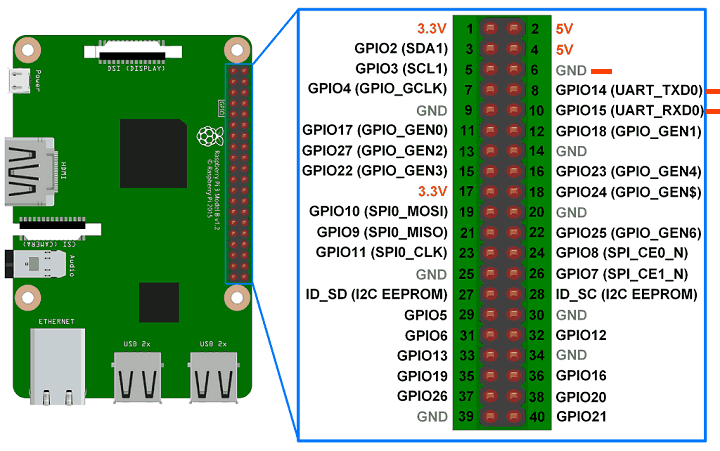
\includegraphics[height=0.4\textheight]{pictures/04_labs/rpi3_gpio_layout_uarts.png} \\
\end{centering}

\begin{center}
  \begin{tabular}{ c | c }
    \hline
    RPi & Connecteur FTDI \\ \hline
    GND - Noir - Pin 6 & GND - Noir \\
    TX - Blanc - Pin 8 & RX - Jaune \\
    RX - Gris - Pin 10 & TX - Orange \\
    \hline
  \end{tabular}
  \end{center}

Ou sur votre RPi avec le module CAN :

\begin{centering}
  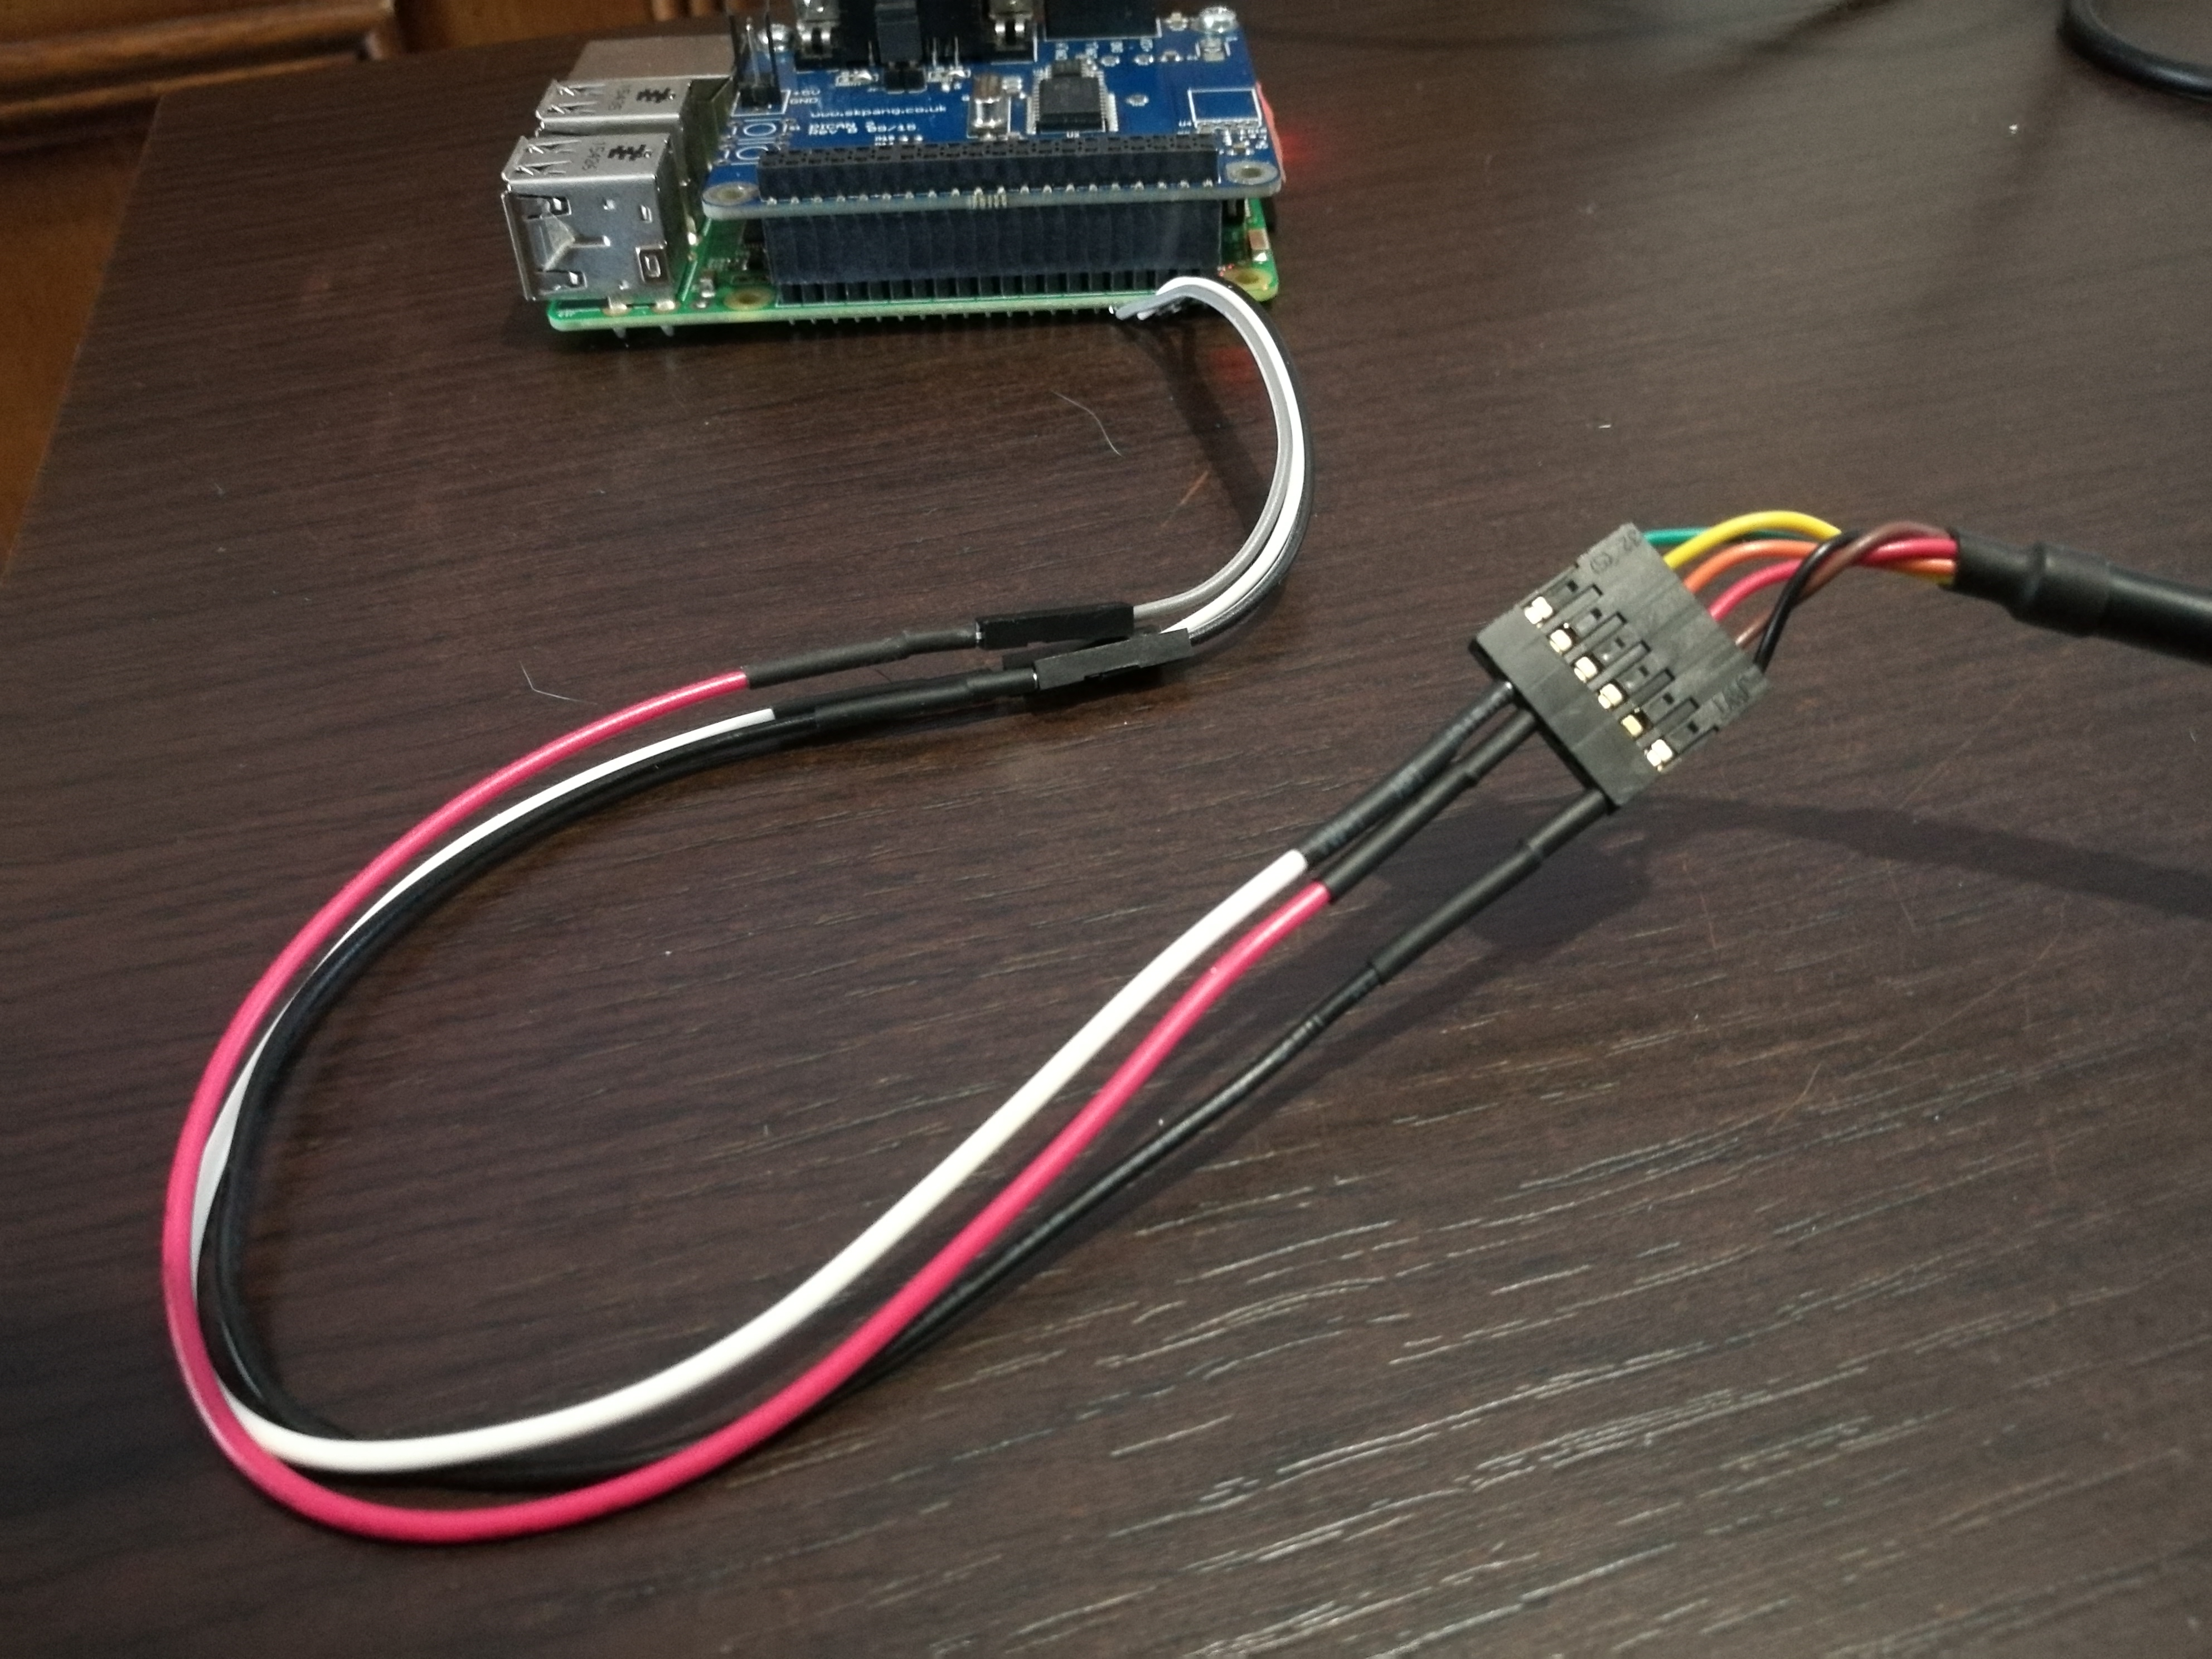
\includegraphics[height=0.3\textheight]{pictures/04_labs/rpi3_pican_uarts.jpg} \\
\end{centering}

Lancer un outils série tel que \texttt{picocom} ou \texttt{gtkterm} :

\begin{verbatim}
picocom -b 115200 /dev/ttyUSB0
\end{verbatim}

Allumez via USB votre board et vous devriez voir le système booter !

Le login est \code{root} et profitez pour explorer le système. Lancer
\code{ps} pour regarder combien de processus sont en cours d'exécution,
qu'est-ce que Buildroot a généré dans \code{/bin}, \code{/lib}, \code{/usr}
et \code{/etc}.

%%%%%%%%%%%%%%%%%%%%%%%%%%%%%%%
\section{Explorer le log de build}
%%%%%%%%%%%%%%%%%%%%%%%%%%%%%%%

De retour sur votre machine de build, regardez la sortie du log \code{build.log}.
Buildroot est un peu verbose mais il affichera chaque message important d'un
prefixe \code{>>>}. Pour avoir une idée générale de ce qui a été fait, vous
pouvez lancer:

\begin{verbatim}
grep ">>>" build.log
\end{verbatim}

Vous voyez les différents paquets être téléchargés, extraits, patchés,
configurés compilés et installés.

\chapter{Ajout du support CAN}
{Objectifs:
  \begin{itemize}
  \item Ajouter de nouveaux paquets à compiler
  \item Configurer un périphérique hardware (CAN) sous la RPi3
  \item Tester le nouveau système
  \end{itemize}
}

\section{Avant de commencer...}

Le controlleur CAN que nous allons utiliser est un
\href{https://www.microchip.com/wwwproducts/en/en010406}{MCP2515} qui utilise
un bus SPI.

Prendre un peu de temps pour lire la datasheet du MCP2515, regarder les
différentes pins, le voltage en entrée, etc. Cela vous permettra de comprendre
les pins suivantes utilisées.

Nous allons utiliser les pins SPI de la RPi : \\

\begin{centering}
  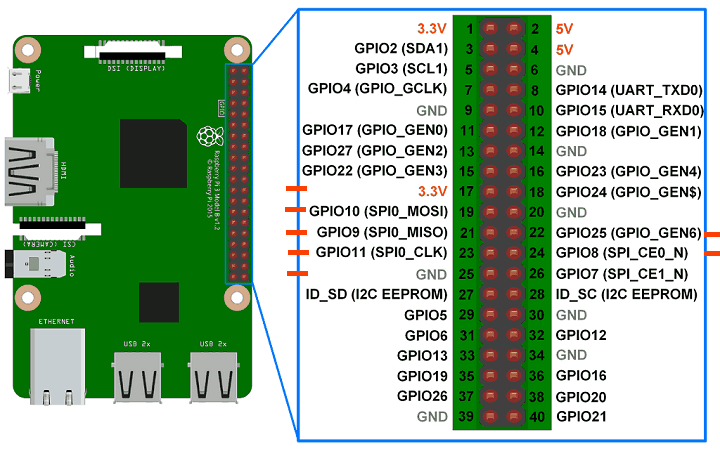
\includegraphics[height=0.3\textheight]{pictures/04_labs/rpi3_gpio_layout_spi.png} \\
\end{centering}

Ce qui nous donnera une connexion SPI suivante : \\

\begin{centering}
  \includegraphics[height=0.3\textheight]{graphics/04_labs/rpi3_mcp2515.pdf} \\
\end{centering}

\section{Configuration}
\subsection{Configuration de la RPi3 : defconfig + device-tree}

Pour ajouter le support d'un périphérique dans Linux, il faut:
\begin{itemize}
\item Ajouter un noeud dans le device tree selon le bus utilisé
\item Activer le driver dans la configuration kernel
\end{itemize}

\subsubsection{Device-tree overlay}

La RPi a une particularité par rapport à certaines cartes de développpement,
elle utilise un fichier de configuration de type texte pour faire des
modifications hardware via un firmware.

Rechercher ce fichier :

\begin{verbatim}
$ find . -iname config.txt
./package/rpi-firmware/config.txt
\end{verbatim}

Lire les fichiers contenus dans le dossier \code{board/raspberrypi3/}.

Regarder comment est-il possible de modifier le fichier \code{config.txt},
notamment avec ce qui est déjà effectué avec l'option \code{dtoverlay=pi3-miniuart-bt}.
Les informations sur la syntaxe de ce fichier sont disponibles sur ce site
\url{http://elinux.org/RPiconfig}. Les dtoverlay permettent d'activer des
parties hardware de la raspberry pi en modifiant le Device Tree.

Pour activer le bus SPI, il faut utiliser le \code{dtparam} et pour activer le
hardware CS, ça sera via \code{dtoverlay} (voir la documentation \href{https://github.com/raspberrypi/firmware/blob/master/boot/overlays/README#L2103..L2106}{ici}):
\begin{verbatim}
dtparam=spi=on
dtoverlay=spi0-hw-cs
\end{verbatim}

En ce qui concerne le chip CAN, il faut utiliser un \code{dtoverlay}.
Voici une \href{https://github.com/raspberrypi/firmware/blob/master/boot/overlays/README#L56}{documentation}
à lire concernant leur utilisation avec la node du controlleur CAN que nous
utiliserons \href{https://github.com/raspberrypi/firmware/blob/master/boot/overlays/README#L1478..L1485}{MCP2515}.
\begin{verbatim}
dtoverlay=mcp2515-can0,oscillator=16000000,interrupt=25
\end{verbatim}

Toutes ces nouvelles valeurs devront être ajoutées dans le fichier \code{config.txt}
en ajoutant du code dans le script \code{post-image.sh} de la RPi3. Prendre
exemple sur les autres arguments pour ajouter une option \code{--add-mcp2515-overlay}.

Une fois que le script a été modifié, il faudra ajouter l'option dans la
configuration Buildroot (cf variable \code{BR2_ROOTFS_POST_SCRIPT_ARGS}).

\begin{centering}
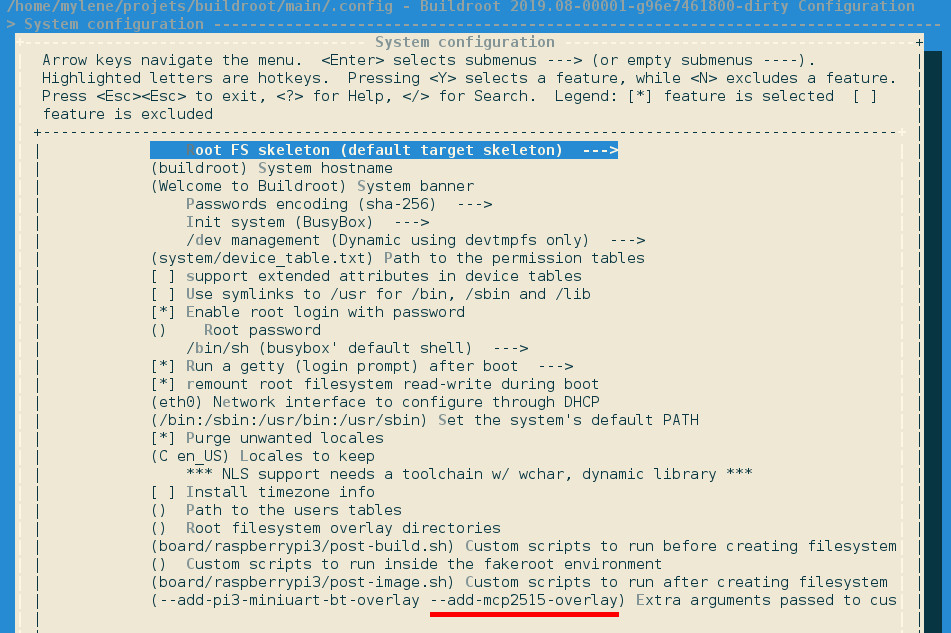
\includegraphics[height=0.3\textheight]{pictures/04_labs/config_br_overlay.jpg} \\
\end{centering}

\subsubsection{Configuration kernel}

Par défaut, le driver pour le controlleur CAN MCP2515 est déjà activé dans
la configuration que l'on utilise du kernel.

Vérifier que la configuration \code{MCP251X} est activée (soit builtin \code{=y}
soit en module \code{=m}) en utilisant la commande suivante :

\begin{verbatim}
make linux-menuconfig
\end{verbatim}

Cela vous ouvrira le menuconfig spécifique au kernel (et non pas à Buildroot).

\subsection{Configuration de Buildroot}

Maintenant que la configuration coté Kernel et device-tree est réalisée, il
faut activer des nouveaux paquets dans Buildroot pour pouvoir avoir des
outils pour utiliser le CAN :
\begin{itemize}
\item \texttt{LIBSOCKETCAN} : Permet de controller un périphérique CAN via du code en C
\item \texttt{CAN\_UTILS} : Permet d'ajouter des outils en ligne de commande pour
  tester des périphériques CAN tel que \code{candump} et \code{cansend}.
\end{itemize}

Ouvrir le menuconfig de buildroot et chercher les paquets qui nous intéressent.
Les activer, sauvegarder votre configuration et compiler une nouvelle image.
Vérifier qu'ils sont bien compilés pour votre RPi3 avec :

\begin{verbatim}
$ find output/target/ -iname can*
\end{verbatim}

\begin{centering}
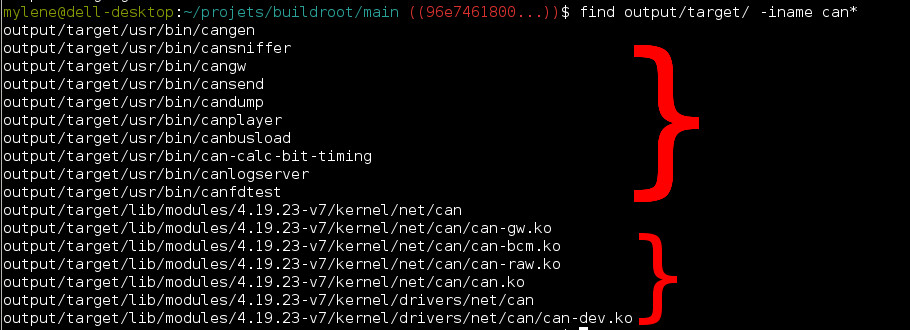
\includegraphics[height=0.2\textheight]{pictures/04_labs/output_target.jpg} \\
\end{centering}

\begin{verbatim}
$ find output/staging/ -iname can*
\end{verbatim}

\begin{centering}
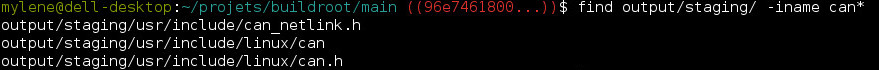
\includegraphics[height=0.05\textheight]{pictures/04_labs/output_staging.jpg} \\
\end{centering}

Maintenant, flasher votre carte SD avec votre nouvelle image, booter votre
RPi3 avec le module CAN connecté comme il faut et tester votre interface
\code{can0} avec :

\begin{verbatim}
$ ip link set can0 up type can bitrate 500000
$ ifconfig
$ cansend can0 01a#11223344AABBCCDD
$ candump can0
\end{verbatim}

%\chapter
{Création d'un nouveau paquet dans Buildroot}
{Objectifs:
  \begin{itemize}
  \item Création d'un nouveau paquet pour {\em nInvaders}
  \item Comprendre comment ajouter des dépendances
  \end{itemize}
}

\section{Préparation}

Après une recherche Google, trouver le site web pour {\em nInvaders}
et télécharger le code source. Analyser son système de build et
déduire quelle infrastructure de paquet est la plus appropriée.

\section{Paquet minimal}

Créer un répertoire pour ce paquet dans les sources de Buildroot :
\code{package/ninvaders}. Créer un fichier \code{Config.in} avec une option
pour activer ce paquet et un fichier \code{ninvaders.mk} minimal qui spécifiera
ce qu'il faut pour juste {\em télécharger} le paquet.

Pour information, l'URL de téléchargement des sources {\em nInvaders} est
\code{http://downloads.sourceforge.net/project/ninvaders/ninvaders/0.1.1/}.

Note: Pour y arriver, seulement deux variables sont nécessaires d'être définies
dans le fichier \code{.mk} ainsi qu'un appel à la macro de l'infrastructure
appropriée.

Maintenant, aller dans le \code{menuconfig}, activer {\em nInvaders}, et lancer
une compilation \code{make}. Vous devriez voir l'archive {\em nInvaders}
être téléchargée et extraite. Regarder dans \code{output/build/} pour voir
si ça a été extrait comme attendu.

\section{C'est parti pour la compilation !}

Comme vous avez pu le voir, {\em nInvaders} utilise un simple \code{Makefile}
pour son processus de build. Vous allez donc devoir définir les variables
de build pour {\em nInvaders}. Pour faire cela, 4 variables sont fournies par
Buildroot :

\begin{itemize}

\item \code{TARGET_MAKE_ENV}, qui devra être passé dans l'environnement utilisé
  lors de la commande \code{make}.

\item \code{MAKE}, contient le vrai appel du \code{make} avec potentiellement
  quelques paramètres pour paralleliser le build.

\item \code{TARGET_CONFIGURE_OPTS}, contient la définition de pleins de
  variables utiles dans les \code{Makefiles} comme : \code{CC},
  \code{CFLAGS}, \code{LDFLAGS}, etc.

\item \code{@D}, contient le chemin vers le répertoire où le code source de
  {\em nInvaders} a été extrait.

\end{itemize}

Quand vous créez des paquets Buildroot, c'est une bonne pratique de regarder
comment les autres paquets sont définis. Regarder par exemple le paquet
\code{jhead} qui sera très similaire à ce dont on a besoin pour notre paquet
\code{ninvaders}.

Lorsque vous avez écrit l'étape de build de {\em nInvaders}, il est temps
de tester! Mais si vous lancez seulement un \code{make} pour redémarrer
un build, le paquet \code{ninvaders} ne sera pas rebuildé car il l'a été
déjà été précemment.

On va donc forcer le build en supprimant complètement le répertoire des
sources :

\begin{verbatim}
make ninvaders-dirclean
\end{verbatim}

Ensuite, recommencer un build :

\begin{verbatim}
make
\end{verbatim}

Cette fois, vous devriez voir l'étape \code{ninvaders 0.1.1 Building} mais
elle échouera car le fichier \code{ncurses.h} est manquant.

\section{Gérer les dépendances}

Le fichier \code{ncurses.h} est manquant parce que {\em nInvaders}
dépends de la bibliothèque \code{ncurses} pour l'interface sur un terminal en
mode "texte". On va donc installer \code{ncurses} comme dépendance de
{\em nInvaders}. Pour cela :

\begin{itemize}

\item Indiquer la dépendance dans le fichier \code{Config.in}. Utiliser le
  \code{select} pour être sûr que le paquet \code{ncurses} sera automatiquement
  sélectionné avec la sélection de \code{ninvaders}.
\item Indiquer la dépendance dans le fichier \code{.mk}.

\end{itemize}

Recommencer un build du paquet avec :
\code{make ninvaders-dirclean all} (qui est pareil que
\code{make ninvaders-dirclean} suivi d'un \code{make}).

Maintenant, le paquet devrait être compilé avec succès !
Si vous jetez un oeil à \code{output/build/ninvaders-0.1.1/}, vous devriez
voir le binaire \code{nInvaders}. Lancer le programme \code{file} sur
\code{nInvaders} pour vérifier que c'est bien pour ARM.

\code{nInvaders} a bien été compilé mais il n'est pas pour autant installé
dans le rootfs de notre cible !

\section{Installation et test du programme}

Si vous regardez le \code{Makefile} des sources de {\em nInvaders},
vous remarquez qu'il n'y a rien pour installer le programme. Il n'y a pas
de règle \code{install:}.

Dans \code{ninvaders.mk}, on va devoir créer une {\em commande d'installation
  pour cible} qui va simplement installer le binaire \code{nInvaders}.
Utiliser la variable \code{$(INSTALL)} pour cela. Regarder le paquet
\code{jhead} comme exemple.

Rebuilder une nouvelle fois \code{ninvaders} et cette fois, vous devriez
voir le binaire \code{nInvaders} dans \code{output/target/usr/bin/}!

Reflasher votre rootfs sur la carte SD et rebooter le système.

\section{Ajout d'un fichier de hash}

Pour finaliser notre paquet, ajouter un fichier manquant : {\em hash file}
pour permettre de vérifier que les personnes builderont les mêmes sources
que celles que vous avez utilisé pour votre paquet. Pour savoir le hash,
SourceForge permet de directement connaitre cela via :
aller dans la page {\em download} et à coté du nom du fichier, il y a une
icône d'information qui vous fournit les hashes MD5 et SHA1.

Recompiler avec \code{make ninvaders-dirclean all}.
Regarder l'output du build et avant le message \code{ninvaders 0.1.1 Extracting},
vous devriez voir :

\begin{verbatim}
ninvaders-0.1.1.tar.gz: OK (sha1: ....)
ninvaders-0.1.1.tar.gz: OK (md5: ....)
\end{verbatim}

\section{Tester la suppression d'un paquet}

Pour jouer un peu avec Buildroot, réaliser les tests suivants : désactiver
le paquet \code{ninvaders} dans le \code{menuconfig} et redémarrer le build via
\code{make}. Quand le build est fini, regarder dans \code{output/target/}.
Est-ce que {\em nInvaders} est toujours installé ? Si oui, pourquoi ?


\end{document}
